%-------------------------------------------------------------------------
\subsection{DECOVALEX HM test case}
\label{sec:thm}

DECOVALEX is an international code comparison project for the verification of thermo-hydro-mechanical (THM) and thermo-hydro-chemical (THC) numerical simulators \cite{BirEtAl:2008} (see also sec. \ref{sec:thc-decovalex}).

\subsubsection*{Definition}

The original DECOVALEX-THM benchmark definition is a 2-D problem \cite{BirEtAl:2008} (Fig. \ref{fig:thm-1D}).
For the comparison of different HM swelling models, we consider a simplified case representing a horizontal cross-section through the 2-D domain (Fig. \ref{fig:thm-1D}, BME1H).

\begin{figure}[!htb]
\includegraphics[width=5cm]{HM/HM_unsat/D-BME.eps}
\caption{2-D DECOVALEX THM definition and simplification for the benchmark exercise BME1H}
\label{fig:thm-1D}
\end{figure}

\begin{figure}[!htb]
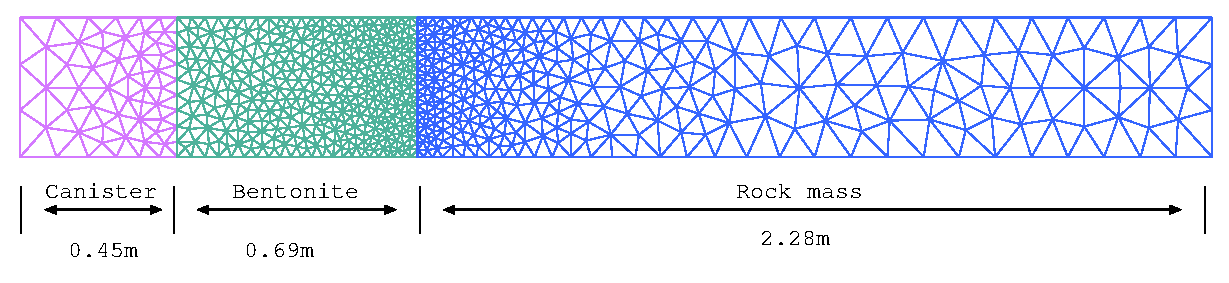
\includegraphics[scale=0.6]{HM/HM_unsat/hm_swelling.eps}
\caption{Mesh of the simplified BME1H model including canister, bentonite, and rock mass sections}
\label{fig:thm-1Dmesh}
\end{figure}

The simplified model takes a rectangle shape. The mesh of the domain together with material types are shown in Fig. \ref{fig:thm-1Dmesh}.

Fig. \ref{fig:BME1H} illustrates the definition of initial and boundary conditions for the horizontal cross-section BME1H.
Observation points are set at $x=0.45\,m, \,x=1.10\,m$ to record temporal breakthrough curves.

\begin{figure}[!htb]
\begin{center}
\footnotesize
% \usepackage[usenames,dvipsnames]{pstricks}
% \usepackage{epsfig}
% \usepackage{pst-grad} % For gradients
% \usepackage{pst-plot} % For axes
% Generated by WW with LaTexDraw
\scalebox{0.8} % Change this value to rescale the drawing.
{
\begin{pspicture}(0,-1.900625)(18.579687,1.900625)
\definecolor{color7g}{rgb}{1.0,0.0,0.2}
\definecolor{color0g}{rgb}{0.4,0.4,0.4}
\definecolor{color0f}{rgb}{0.6,0.6,0.6}
\psframe[linewidth=0.04,dimen=outer,fillstyle=gradient,gradlines=2000,gradbegin=color0g,gradend=color0f,gradmidpoint=1.0](12.799687,1.0171875)(1.7796875,-1.1428125)
\psframe[linewidth=0.04,dimen=outer,fillstyle=gradient,gradlines=2000,gradbegin=color7g,gradend=color7g,gradmidpoint=1.0](3.7996874,1.0171875)(1.7596875,-1.1228125)
\psframe[linewidth=0.04,dimen=outer,fillstyle=gradient,gradlines=2000,gradbegin=blue,gradend=blue,gradmidpoint=1.0](6.4396877,1.0171875)(3.7796874,-1.1428125)
\psframe[linewidth=0.04,dimen=outer](18.539688,1.4571875)(18.519688,1.2971874)
\usefont{T1}{ptm}{m}{n}
\rput(7.403125,1.5271875){$u_y$=0, $\sigma_{xy}$=0}
\usefont{T1}{ptm}{m}{n}
\rput(7.383125,-1.6728125){$u_y$=0, $\sigma_{xy}=0$}
\usefont{T1}{ptm}{m}{n}
\rput(14,0.2471875){$u_x=0, \sigma_{xy}=0$}
\usefont{T1}{ptm}{m}{n}
\rput(13.8,-0.1){$p^l=10^6$Pa}
\usefont{T1}{ptm}{m}{n}
\rput(0.973125,0.2471875){$u_x$=0}
\usefont{T1}{ptm}{m}{n}
\rput(0.99,-0.1){$\sigma_{xy}$=0}
\usefont{T1}{ptm}{m}{n}
\rput(5.,0.24){\color{red}S0=0.65}
\usefont{T1}{ptm}{m}{n}
\rput(5.1,-0.1){\color{yellow}($p^l=-7\times10^7$Pa)}
\usefont{T1}{ptm}{m}{n}
\rput(9,-0.1728125){\color{yellow}$p^l=10^5$Pa}
\end{pspicture}
}
\caption{Simplified horizontal cross-section model}
\label{fig:BME1H}
\end{center}
\end{figure}

The material parameters for rock mass and bentonite are given in
Table \ref{tab:hm_rock} and \ref{tab:hm_bentonite},
respectively.

\begin{table}[!thb]
\begin{center}
\begin{tabular}{lll}
\hline \hline
Parameter   &  Unit  & Value\\
\hline \hline
 Density &  $kg/m3$ &  2700 \\
 Young's modulus &  $GPa$ &  $35$ \\
 Poisson ratio & - &  0.3 \\
 Porosity & - &  0.01 \\
 Saturated permeability &  $m2$  & $1.0
\times10^{-17}$ \\
\hline \hline
\end{tabular}
\end{center}
\caption{\label{tab:hm_rock}Rock Mass}

\end{table}
%%%%%
\begin{table}[!thb]
\begin{center}
\begin{tabular}{lll}
\hline \hline
 Density &  $kg/m3$ &  1600 \\
 Young's modulus &  $MPa$ &  $317$\\
 Poisson ratio & - &  0.35 \\
 Saturated permeability &  $m2$  & $2.0
\times10^{-21}$ \\
\hline \hline
\end{tabular}
\end{center}
\caption{\label{tab:hm_bentonite}Bentonite}
\end{table}

The dependency of capillary pressure
as well as relative permeability on liquid saturation for both of
rock and bentonite are depicted in Fig. \ref{fig:cp_cp}.

\begin{figure}[!htb]
  \begin{center}
    \begin{minipage}[t]{0.45\textwidth}
      \begin{center}
        \includegraphics[scale=0.27]{HM/HM_unsat//capsat_new.eps}\\
        \centerline{Capillary pressure}
      \end{center}
    \end{minipage}
  %%\hspace{0.01\textwidth}
    \begin{minipage}[t]{0.45\textwidth}
      \begin{center}
        \includegraphics[scale=0.27]{HM/HM_unsat/persat.eps}\\
        \centerline{Relative permeability}
      \end{center}
    \end{minipage}\\
  \end{center}
  \caption{Capillary pressure - relative permeability - functions}
  \label{fig:cp_cp}
\end{figure}


\subsubsection*{Results}

Fig. \ref{fig:hmswl_cont} displays a contour plot of saturation and vertical swelling stress in the domain. Apparently, the swelling stress in the bentonite is induced by change of water saturation.
\begin{figure}[!htb]
\centering
\includegraphics[scale=0.5]{HM/HM_unsat/swelling_cont.eps}
\caption{Distribution of saturation and vertical swelling stress}
\label{fig:hmswl_cont}
\end{figure}

Fig. \ref{fig:deco-hm} shows the simulated horizontal profiles (top) and temporal evolutions at observation point (bottom) of water saturation and swelling stress based on the linear swelling model (\ref{eqn:swelling}) proposed by Rutqvist (2005) \cite{Jonny05}.

\begin{figure}[!htb]
\begin{center}
\includegraphics[width=9cm]{HM/HM_unsat/LinearSwellingH.eps}
\includegraphics[width=9cm]{HM/HM_unsat/LinearSwellingTime.eps}
\caption{Horizontal profile (top) and temporal evolution at observation point (bottom) of water saturation and swelling stress}
\label{fig:deco-hm}
\end{center}
\end{figure}

\subsubsection*{Benchmark deposit}
\begin{tabular}{|l|l|l|}
  \hline
  Benchmark & Problem type & Path in benchmark deposit \\
  \hline
 \emph{hm\_swelling}& HM &  HM/LinearSwelling\\
  \hline
\end{tabular}






